\documentclass[border=12pt]{standalone}
\usepackage{tikz}
\usetikzlibrary{arrows.meta,calc}

\definecolor{spherefill}{RGB}{235,242,250}
\definecolor{sphereedge}{RGB}{70,90,120}
\definecolor{axiscolor}{RGB}{40,40,45}
\definecolor{statevec}{RGB}{180,45,45}
\definecolor{arccolor}{RGB}{50,110,160}
\definecolor{labelgray}{RGB}{60,60,65}

\begin{document}
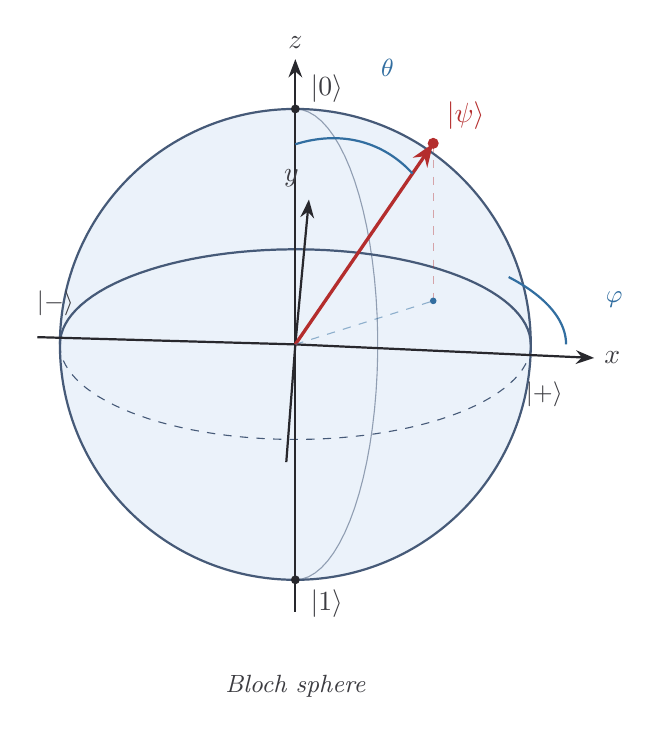
\begin{tikzpicture}[x=1.15cm,y=1.15cm,>=Stealth]
  % --- ellipse parameters (2D projection of sphere) ---
  % equatorial ellipse: a=2.6 (x), b=1.05 (depth)
  \def\Rx{2.6}
  \def\Ry{1.05}
  \def\Rz{2.6}

  % sphere body (front fill)
  \fill[spherefill] (0,0) circle (\Rx);
  \draw[sphereedge,thick] (0,0) circle (\Rx);

  % hidden (back) equator arc -- dashed
  \draw[sphereedge,dashed,thin]
    plot[domain=180:360,samples=60]
      ({\Rx*cos(\x)},{\Ry*sin(\x)});

  % visible (front) equator arc
  \draw[sphereedge,thick]
    plot[domain=0:180,samples=60]
      ({\Rx*cos(\x)},{\Ry*sin(\x)});

  % meridian (front vertical great circle hint)
  \draw[sphereedge,thin,opacity=0.55]
    plot[domain=-90:90,samples=40]
      ({\Rx*0.35*cos(\x)},{\Rz*sin(\x)});

  % --- axes ---
  % z axis (vertical)
  \draw[axiscolor,thick,->]
    (0,-\Rz-0.35) -- (0,\Rz+0.55)
    node[above,labelgray] {$z$};
  % x axis (to the right, slightly down for perspective)
  \draw[axiscolor,thick,->]
    (0,0) -- ({\Rx+0.7},{-0.15})
    node[right,labelgray] {$x$};
  % y axis (into page / depth, along ellipse minor)
  \draw[axiscolor,thick,->]
    (0,0) -- ({0.15},{\Ry+0.55})
    node[above left,labelgray,yshift=1pt] {$y$};
  % negative axis stubs
  \draw[axiscolor,thick]
    (0,0) -- ({-\Rx-0.25},{0.08});
  \draw[axiscolor,thick]
    (0,0) -- ({-0.1},{-\Ry-0.25});

  % poles
  \fill[axiscolor] (0,\Rz) circle (1.6pt)
    node[above right,labelgray,xshift=2pt,yshift=-1pt]
      {$|0\rangle$};
  \fill[axiscolor] (0,-\Rz) circle (1.6pt)
    node[below right,labelgray,xshift=2pt]
      {$|1\rangle$};

  % equator basis hints
  \node[labelgray,font=\small] at ({\Rx+0.15},{-0.55})
    {$|+\rangle$};
  \node[labelgray,font=\small] at ({-\Rx-0.05},{0.45})
    {$|-\rangle$};

  % --- state vector |psi> ---
  % choose theta ~ 50 deg, phi ~ 40 deg (visual)
  % projection: r_xy = R * sin(theta)
  % x' = r_xy * cos(phi), y' = r_xy * sin(phi) * (Ry/Rx aspect)
  % z' = R * cos(theta)
  \def\thetaval{48}
  \def\phival{38}
  \pgfmathsetmacro{\psix}{\Rx*sin(\thetaval)*cos(\phival)}
  \pgfmathsetmacro{\psiy}{\Ry*sin(\thetaval)*sin(\phival)}
  \pgfmathsetmacro{\psiz}{\Rz*cos(\thetaval)}
  % combine: horizontal = psix, vertical = psiz + psy (depth tilt)
  \pgfmathsetmacro{\psiX}{\psix}
  \pgfmathsetmacro{\psiY}{\psiz + \psiy}

  % radial guide (dashed) from origin to state
  \draw[statevec,opacity=0.35,dashed,thin]
    (0,0) -- (\psiX,\psiY);

  % state vector arrow
  \draw[statevec,very thick,->]
    (0,0) -- (\psiX,\psiY)
    node[above right,statevec,xshift=1pt,yshift=1pt]
      {$|\psi\rangle$};

  % tip marker
  \fill[statevec] (\psiX,\psiY) circle (2pt);

  % projection onto xy-plane (equator disk)
  \pgfmathsetmacro{\projX}{\Rx*sin(\thetaval)*cos(\phival)}
  \pgfmathsetmacro{\projY}{\Ry*sin(\thetaval)*sin(\phival)}
  \draw[statevec,opacity=0.4,dashed,thin]
    (\psiX,\psiY) -- (\projX,\projY);
  \draw[arccolor,opacity=0.5,dashed,thin]
    (0,0) -- (\projX,\projY);
  \fill[arccolor] (\projX,\projY) circle (1.2pt);

  % --- theta arc (from +z toward |psi>) ---
  % small arc in the plane containing z and |psi>
  \draw[arccolor,thick]
    plot[domain=0:\thetaval,samples=40]
      ({0.85*\Rx*sin(\x)*cos(\phival)},
       {0.85*\Rz*cos(\x) + 0.85*\Ry*sin(\x)*sin(\phival)});
  \node[arccolor,font=\small]
    at
    ({1.15*\Rx*sin(\thetaval*0.45)*cos(\phival)+0.15},
     {1.15*\Rz*cos(\thetaval*0.45)
      +1.15*\Ry*sin(\thetaval*0.45)*sin(\phival)})
    {$\theta$};

  % --- phi arc (on equatorial plane, from +x toward projection) ---
  \draw[arccolor,thick]
    plot[domain=0:\phival,samples=30]
      ({1.15*\Rx*cos(\x)},{1.15*\Ry*sin(\x)});
  \node[arccolor,font=\small]
    at ({1.45*\Rx*cos(\phival*0.55)},
        {1.45*\Ry*sin(\phival*0.55)-0.05})
    {$\varphi$};

  % title-ish caption (textbook quiet)
  \node[labelgray,font=\small\itshape,anchor=north]
    at (0,-\Rz-0.95)
    {Bloch sphere};

\end{tikzpicture}
\end{document}
